%%=============================================================================
%% Conclusie
%%=============================================================================

\chapter{Conclusie}%
\label{ch:conclusie}

% TODO: Trek een duidelijke conclusie, in de vorm van een antwoord op de
% onderzoeksvra(a)g(en). Wat was jouw bijdrage aan het onderzoeksdomein en
% hoe biedt dit meerwaarde aan het vakgebied/doelgroep? 
% Reflecteer kritisch over het resultaat. In Engelse teksten wordt deze sectie
% ``Discussion'' genoemd. Had je deze uitkomst verwacht? Zijn er zaken die nog
% niet duidelijk zijn?
% Heeft het onderzoek geleid tot nieuwe vragen die uitnodigen tot verder 
%onderzoek?

Op basis van de resultaten in hoofdstuk 4 van deze studie kunnen we de initiële onderzoeksvragen beantwoorden in de 
conclusies van deze proef.

\section{\IfLanguageName{dutch}{Conclusie van pentesttools}{conclusion of pentesttools}}
  Welke penetratietesttool(s) zijn volgens de vooraf bepaalde criteria het meest effectief en efficiënt in het 
  identificeren van kwetsbaarheden in de drie specifieke webomgevingen.  
  De prestaties van de penetratietesttools Burp Suite, Metasploit en OWASP ZAP varieerden bij het onderzoeken van de 
  meest effectieve tool voor het identificeren van kwetsbaarheden in de drie geselecteerde webomgevingen.

  Bij het bepalen van de effectivivteit van de tools kwam OWASP ZAP naar boven als meest gepaste keuze op basis van de richtlijnen 
  die vooraf werden opgesteld in deze studie. OWASP ZAP scoorde tevens hoog op het gebied van scala aan functionaliteiten, 
  ondersteuning van de community en gebruiksvriendelijkheid. De open-source aard van OWASP ZAP maakt het een aantrekkelijke 
  keuze voor organisaties met beperkte budgetten voor beveiligingstests. Burp Suite en Metasploit scoorden respectievelijk 
  lager op het gebied van gebruiksvriendelijkheid en kosten en bieden een minder uitgebreide reeks van functionaliteiten en 
  ondersteuning van de community. Deze conclusie is ook terug te vinden in de resultaten van de penetratietest tools 
  \nameref{sec:Definitieve_pentesttool}.

  \section{\IfLanguageName{dutch}{Conclusie van webomgevingen}{Conclusion of web environments}}  
   Welke specifieke kwetsbaarheden detecteren de penetratietesttools in een WordPress-omgeving zonder beveiligingsplugins en 
   hoe verschillen deze van testen op de omgevingen met beveiligingsplugins en de Laravel-applicatie.
  
  In een WordPress-omgeving zonder beveiligingsplugins werden meerdere kwetsbaarheden blootgelegd door penetratietests en 
  externe onderzoeken. De meest voorkomende kwetsbaarheden waren gerelateerd aan zwakke wachtwoorden, onbeperkte 
  inlogpogingen, en ontbrekende beveiligingsmaatregelen. Beveiligingsplugins, zoals Wordfence, lieten een aanzienlijke 
  verbetering zien in het detecteren en blokkeren van aanvallen. De ingebouwde beveiligingsmaatregelen, zoals geavanceerde 
  gebruikersauthenticatie en versleutelingstechnieken, boden een solide bescherming.

  Uit de uitgevoerde tests bleek dat de voornaamste kwetsbaarheden vaak samenhangen met de manier waarop een omgeving is 
  ingesteld. Bij het opzetten van een omgeving moet er een afweging worden gemaakt tussen zichtbaarheid en bruikbaarheid op het 
  internet en veiligheid. Het is daarom belangrijk om duidelijk te bepalen waarvoor een webomgeving wordt gebruikt en welke 
  gegevens erin worden opgeslagen.

  Een WordPress-omgeving met beveiligingsplugins is een omgeving die snel en gemakkelijk kan worden opgezet en waarbij 
  zichtbaarheid op het web belangrijk is. Het is hierbij essentieel om de juiste beveiligingsplugins te installeren en de 
  omgeving zorgvuldig te configureren.

  De conclusie die hieruit kan worden getrokken, is dat Laravel- en WordPress-applicaties met beveiligingsplugins voor 
  verschillende doeleinden worden gebruikt. Een Laravel-omgeving is bijvoorbeeld geschikt voor op maat gemaakte applicaties, 
  waarbij de beveiliging in detail kan worden aangepast aan de specifieke behoeften dit wordt door de ontwikkelaar zelf 
  ingesteld. In tegenstelling tot WordPress, waarbij de beveiliging voornamelijk wordt bepaald door de beveiligingsplugins 
  die worden geïnstalleerd door de eigenaar van de website.

  \section{\IfLanguageName{dutch}{scores van pentests op webomgevingen}{scores of pentests on web environments}}  
  \begin{figure}
    \centering
    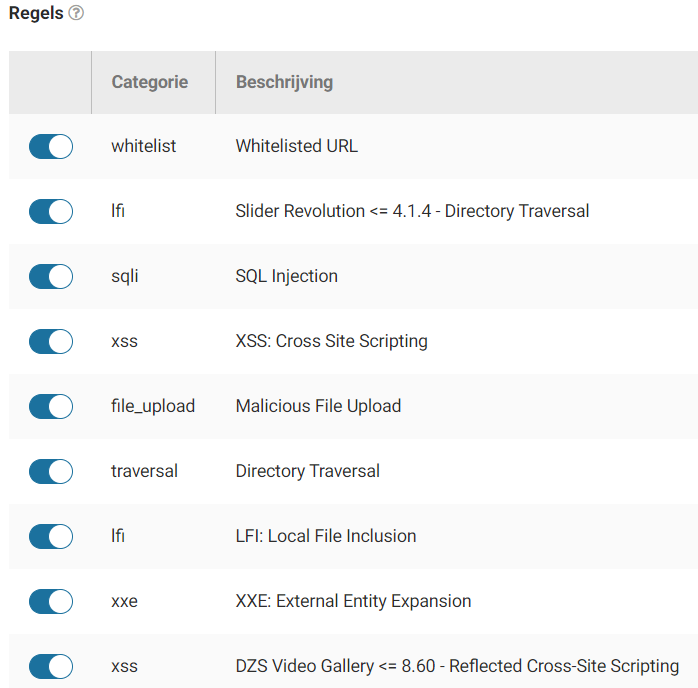
\includegraphics[height=0.3\textheight]{wordfence_regels.png}
    \caption[Bijkomende regels die worden ingesteld door de wordfence plugin]{Bijkomende regels die worden ingesteld door de wordfence plugin}
    \label{fig:wordfence_regels}
  \end{figure}

  \begin{itemize}
    \item Conslusie SQL-injectie:
    \begin{enumerate}
      \item Laravel: 0/15 mogelijke kwetsbaarheden
      \item WordPress met beveiligingsplugins: 4/15 mogelijke kwetsbaarheden
      \item Wordpress zonder beveiligingsplugins: 15/15 mogelijke kwetsbaarheden
    \end{enumerate}
    \item Security misconfiguration:
    \begin{enumerate}
      \item Laravel: kwetsbaarheid op vlak van update/upgrade meldingen
      \item WordPress met beveiligingsplugins: geen mogelijke kwetsbaarheden
      \item Wordpress zonder beveiligingsplugins: kwetsbaarheid op vlak van update/upgrade meldingen \& meldingen bij 
            foutieve wachtwoord en correcte gerbuikersnaam.
    \end{enumerate}
    \item Sensitive data exposure: Dit is een kwetsbaarheid die niet werd gedetecteerd door de tools, maar door de 
          externe testen in verband met de server en database. De conclusie hierbij is voor elke tool hetzelfde, doordat dit 
          regels zijn die ingetseld kunnen worden op de server.
    \item Cross-site scripting (XSS): Hierbij is de gedetecteerde vulnerability de optie van een instelling in de 
          server. De conclusie hierbij is voor elke tool hetzelfde, maar bij wordperss omgeving met beveiligingsplugins 
          zijn er minder mogelijkheden om deze kwetsbaarheid te exploiteren aangezien er aditionele regels zijn ingesteld 
          via de wordfence plugin \ref{fig:wordfence_regels}.
    \item Onvoldoende logging en monitoring: Dit is een kwetsbaarheid die niet werd gedetecteerd door de tools, maar door 
          externe testen op de server. De conclusie hierbij is voor elke tool hetzelfde. Ook hierbij is het door instellingen 
          op de server dat deze kwetsbaarheid kan worden opgelost.
    \item Brute force aanvallen:
    \begin{enumerate}
      \item Laravel: na 4 pogingen wordt de account tijdelijk geblokkeerd
      \item WordPress met beveiligingsplugins: na 5 pogingen wordt de account tijdelijk geblokkeerd
      \item Wordpress zonder beveiligingsplugins: onbeperkte inlogpogingen
    \end{enumerate}
  \end{itemize}

  Samenvattend toont het onderzoek aan dat beveiligingsplugins een cruciale rol spelen in het versterken van de 
  beveiliging van WordPress-omgevingen, waardoor de detectie en blokkering van aanvallen aanzienlijk verbeteren. De keuze 
  van penetratietesttools moet zorgvuldig worden afgestemd op de specifieke behoeften en de complexiteit van de te testen 
  omgeving. Laravel-applicaties profiteren van hun robuuste ingebouwde beveiligingsarchitectuur, wat ze merkbaar veiliger 
  maakt in vergelijking met standaard WordPress-omgevingen.

  Daarnaast speelt de gebruiksvriendelijkheid van de tools een belangrijke rol, waarbij OWASP ZAP opvalt als een intuïtieve 
  en kosteneffectieve optie voor beveiligingstests. Het serveraspect van de omgeving is eveneens van groot belang en mag niet 
  over het hoofd worden gezien bij het opzetten van een webomgeving
